% Track-confirmation matched-control study — ICCV submission draft (rewritten 2026-08-03)
% Compile: pdflatex main.tex && bibtex main && pdflatex main.tex && pdflatex main.tex
% (drop in the official author-kit style; falls back to a plain two-column
% article so the draft builds standalone). The shared CVPR/ICCV author kit
% (https://github.com/cvpr-org/author-kit) ships the style as cvpr.sty, not
% iccv.sty, for both venues.
\IfFileExists{cvpr.sty}{%
  \documentclass[10pt,twocolumn,letterpaper]{article}
  \usepackage[review]{cvpr}
  % cvpr.sty's review-mode watermark requires these to be defined.
  \def\paperID{0000}
  \def\confName{ICCV}
  \def\confYear{2027}
}{%
  \documentclass[10pt,twocolumn,letterpaper]{article}
  \usepackage[margin=2cm]{geometry}
}
\usepackage{graphicx}
% cvpr.sty inlines everyshi's commands unguarded; mark the package as loaded
% so pgf does not load the real one on top and redefine them.
\expandafter\def\csname ver@everyshi.sty\endcsname{2001/05/15}
\usepackage{tikz}
\usepackage{pgfplots}
\pgfplotsset{compat=1.15}
\usepackage{amsmath,amssymb}
\usepackage{booktabs}
\usepackage{multirow}
\usepackage[breaklinks,colorlinks]{hyperref}

% Global custom macro definitions only — see CLAUDE.md split rules.


\begin{document}

\title{Retrospective Confirmation for Identity-Consistent
Streaming 3D Perception}

\author{Anonymous ICCV submission\\Paper ID 0000}
\maketitle

\begin{abstract}
Streaming 3D perception systems emit objects whose identities and class labels
flicker: the same physical object is re-detected as a new instance, or changes
class, from one frame to the next. We present a training-free
\emph{retrospective confirmation} module that runs on frozen detector output
and changes no box coordinate, score, or label. A track is emitted only after
$N$ observations, the standard confirmation test; at confirmation the module
retrospectively releases the withheld prefix, a step online trackers omit,
recovering the trajectory whole. Because such a rule also reduces how much a
system emits, and most metrics respond to volume alone, we validate it against
\emph{matched controls}: a score threshold at the identical detection count,
and a top-$K$ selection at the identical identity count. On nuScenes with a
frozen detector, association accuracy improves against every control in both
association frames ($\mathrm{AssA}\,{+}0.049$ in the sensor frame), with
bootstrap intervals excluding zero. On ScanNet200 --- an indoor
open-vocabulary pipeline sharing no detector, modality, or codebase --- the
same module reduces class-label switching by $26.9\%$ against an
identity-matched control, with segmentation accuracy unchanged. The gain is in
consistency specifically, and it is paid for in detection recall and in
$N{-}1$ frames of latency.
\end{abstract}

\section{Introduction}
\label{sec:intro}

Streaming 3D perception systems --- detectors and semantic mappers that run on
a live sensor feed~\cite{streamingperception,streaming3d,conceptfusion,conceptgraphs}
--- are consumed downstream as \emph{persistent objects}: a map, a scene
graph, a planner's object memory. What those consumers need is that one
physical object stay one object with one label. What streaming systems
actually produce flickers, because the prevailing emission rule is a per-frame
confidence threshold: every detection above a score cut-off enters the stream
immediately, independently of what was emitted a frame earlier. A re-detected
object arrives as a new identity, and an unstable open-vocabulary label changes
class along the way. Per-frame detection metrics do not see this, and so do not
penalise it. Temporal remedies exist --- confirmation counts, and confidence
accumulated along a track~\cite{cbmot,simpletrack,polymot,fastpoly} --- but
each also reduces how much a system emits, and detection-oriented metrics are
strongly coupled to output volume, so a comparison that does not hold that
volume fixed reports what a rule \emph{selects} and how much it \emph{removes}
together. The property is thus both unmeasured by the dominant metrics and
unattributed by the dominant comparison.

We study a \emph{retrospective confirmation} module in that setting, requiring
no retraining and no change to the perception model. Detections are linked into
tracks by a class-agnostic associator; a track becomes \emph{confirmed} only
after $N$ observations, and at that moment the module emits not only the
current detection but the track's withheld prefix, so a confirmed object's
trajectory is complete from its first observation. Nothing about a box's
coordinates, score, or label is modified, and the module runs at a single
operating point ($N{=}3$) with no per-dataset or per-metric tuning.

The attribution problem applies to our module as much as to any other, so we
evaluate under \emph{matched controls} that hold the output budget fixed while
the selection rule varies. A \emph{detection-budget-matched} control thresholds
the same frozen detector output to emit exactly as many detections as the
module; an \emph{identity-budget-matched} control keeps, per sequence, the
highest-scoring $K$ tracks, where $K$ is the number of identities the module
emits. To compare persistence against the other established temporal rule
rather than against score alone, a third control accumulates confidence along a
track in the manner of CBMOT~\cite{cbmot} and is held to both budgets. All
controls share the detector, the association step, and the evaluation code with
the module, differing only in the rule that selects what is emitted.

Under these controls, on the nuScenes validation set (150 scenes, a frozen
CenterPoint~\cite{centerpoint} detector, both sensor-frame and ego-motion-%
compensated world-frame association, confirmed tracks emitted
retrospectively), the module improves association accuracy (HOTA's AssA
component~\cite{hota}) over both matched controls in both association frames,
with bootstrap confidence intervals excluding zero, while class-aware tracking
accuracy AMOTA~\cite{nuscenes_tracking} --- a point estimate, since it does not
admit the same per-scene resampling --- rises consistently in sign and
magnitude. At the same output budget it \emph{reduces} per-frame detection
quality (Sec.~\ref{sec:detmatch}). The gain is bought rather than added.

Against confidence accumulation this becomes the paper's central observation:
at a matched budget the two temporal rules do not order one another but sit at
different points of the same trade-off. Persistence yields higher association
accuracy, accumulation retains the advantage on the detection- and
identity-oriented measures, and each of these differences has an interval
excluding zero. The separation is the same size whether emitted
\emph{detections} or emitted \emph{identities} are held fixed, which rules out
the simplest explanation --- that persistence gains association accuracy merely
by carrying fewer identities to confuse.

Because the module touches only emission timing, it transfers to any streaming
pipeline that re-observes objects. We apply the identical module, unchanged
and at the same $N$, to an indoor open-vocabulary instance-segmentation
pipeline that shares no detector, modality, or codebase with the outdoor one,
and evaluate it under the same control design. On ScanNet200 (312 validation
scenes, 3D instance-mask proposals labeled per frame by a 2D open-vocabulary
detector), the module reduces the number of frames in which an instance's
class label changes by 26.9\% relative to an identity-budget-matched control
of equal size, while leaving instance-segmentation AP essentially unchanged. The
temporal system has fewer label switches in 309 of 312 scenes and the paired
confidence interval excludes zero by a wide margin, whereas selecting the same
number of instances at random reproduces none of the reduction --- so the gain
is specific to temporal selection rather than to emitting fewer identities.

\noindent\textbf{Contributions.}
\begin{itemize}\itemsep2pt
\item \textbf{A training-free retrospective confirmation module.} An operator
combining the standard confirmation test with retrospective emission of the
confirmed prefix, applied to frozen detector output at a single operating
point, with no retraining, no architectural change, and no modification of box
coordinates, scores, or labels.
\item \textbf{The retrospective emission policy, isolated.} We show the
retrospective step is what completes the module: emitting causally instead
narrows \emph{where} the gain holds --- it survives in the sensor frame but
reverses in the world frame --- and retrospection's price is $N{-}1$ frames
of latency ($1.0$\,s at $2$\,Hz for $N{=}3$).
\item \textbf{A matched-budget comparison of two temporal selection rules.}
Confirmation and confidence accumulation are compared at an identical emission
budget and again at an identical identity budget, with paired per-sequence
statistics. Neither dominates: persistence buys association accuracy,
accumulation keeps the detection- and identity-oriented measures, and the
separation is unchanged under either matching.
\item \textbf{Controls that separate a rule from its suppression.} Both budgets
are also matched against a non-temporal score threshold, and indoors against
random selection, so what the comparisons credit is the selection rule rather
than the smaller volume it emits. The design is not specific to confirmation
and applies to any component that alters output volume.
\item \textbf{Cross-domain validation under that design.} Outdoors, the
module improves association accuracy and class-aware tracking accuracy under
both controls in both association frames, at a detection cost we quantify in
Sec.~\ref{sec:detmatch} rather than leave implicit. Indoors, the identical module
reduces class-label switching on an unrelated open-vocabulary
instance-segmentation pipeline, with segmentation quality unchanged.
\end{itemize}

\section{Related Work}
\label{sec:related}

\noindent\textbf{Streaming perception.} Streaming perception was formalised
by~\cite{streamingperception}, which scores predictions against the world at
the moment they are \emph{emitted}, folding latency and accuracy into streaming
AP (sAP); later work optimises detectors for this
regime~\cite{streamyolo}, and the 3D analogue processes LiDAR sectors as they
arrive rather than waiting for a full sweep~\cite{streaming3d}. This line
establishes our premise but corrects \emph{when} a prediction is scored: sAP
remains a per-frame average precision, so two systems emitting identical boxes
at identical latency but differing entirely in identity continuity and label
stability receive the same sAP. We hold latency and box geometry fixed and ask
what that family cannot see.

\noindent\textbf{Track lifecycle and confirmation.} Deciding when a candidate
track is real enough to report is among the oldest problems in multi-target
tracking. The classical radar literature settles it with \emph{track
confirmation} --- under $M$-out-of-$N$ history logic a track is confirmed once
it has been assigned a detection in $M$ of the last $N$ updates, under score
logic once its likelihood ratio crosses a sequential threshold --- and designs
confirmation, deletion, and track management together~\cite{blackmanpopoli}.
The same literature established that reporting may lag estimation:
\emph{retrodiction} revises earlier estimates once later measurements arrive,
in exchange for a bounded delay~\cite{retrodiction}. Tracking-by-detection
inherited the count-based half: SORT~\cite{sort} and DeepSORT~\cite{deepsort}
withhold a tentative track until matched in $N$ consecutive frames, and
AB3DMOT~\cite{ab3dmot} carries the same minimum-hits rule onto 3D boxes, while
CenterPoint~\cite{centerpoint} keeps a max-age deletion rule but reports tracks
from their first observation. None of this is ours: the confirmation test we
use is the textbook one at its conventional operating point. Our retrospective
emission likewise buys completeness with delay, as fixed-lag smoothing does,
and differs in what it revises --- it releases a confirmed track's withheld
prefix with coordinates, scores, and labels exactly as the detector produced
them, so the backward step changes set \emph{membership}, not state.

\noindent\textbf{Confidence in the track lifecycle.} Recent 3D tracking has
largely moved this decision from counting to confidence.
CBMOT~\cite{cbmot} replaces the minimum-hits criterion outright, propagating a
tracklet score by constant decay, fusing it probabilistically with each matched
detection score, and gating both output and termination on the refined score;
it reports consistent AMOTA gains over count-based lifecycles.
SimpleTrack~\cite{simpletrack} decomposes tracking-by-detection into
pre-processing, association, motion model, and lifecycle management, and names
\emph{output} as a lifecycle decision separate from birth and death, letting
low-score detections sustain a track through association without being emitted.
Poly-MOT~\cite{polymot} and Fast-Poly~\cite{fastpoly} pair category-specific
association with mixed count- and confidence-based termination and explicit
control over which trajectories are written out; Fast-Poly adopts CBMOT's
score-fusion rule directly. Confidence-based temporal management is therefore
established and well tuned, and we treat it as such: our contribution is not a
new confirmation or lifecycle mechanism, and our associator is deliberately
lightweight, so our absolute tracking scores are not comparable to these
systems'. What we take from this line is a comparison rather than a competitor.
Persistence-based confirmation and confidence accumulation are two temporal
rules that both decide which detections reach the output, and both reduce how
much is emitted; since detection-oriented metrics are strongly coupled to
output volume, a comparison that does not hold that volume fixed reports the
suppression and the rule together. Budget-matched comparison is routine when
scoring detectors at a fixed proposal count; we apply it to temporal selection,
holding fixed each of the two currencies such a rule spends --- emitted
detections and emitted identities --- and read what separates the two rules
under each.

\noindent\textbf{Open-vocabulary 3D perception.} OpenScene~\cite{openscene}
distils 2D vision--language features into 3D points and LERF~\cite{lerf} embeds
language into a radiance field; OpenMask3D~\cite{openmask3d} moves to instances
via per-mask CLIP features over class-agnostic 3D proposals, and
Open-YOLO~3D~\cite{openyolo3d} replaces that extraction with 2D
open-vocabulary boxes projected onto 3D masks. All four are \emph{offline},
consuming a completed reconstruction. ConceptFusion~\cite{conceptfusion} and
ConceptGraphs~\cite{conceptgraphs} make the setting incremental, merging
per-frame detections into persistent object nodes. A more recent line segments
3D instances fully online, computing proposals per frame:
EmbodiedSAM~\cite{embodiedsam} lifts per-frame 2D masks into 3D queries matched
across views by a learned similarity, OnlineAnySeg~\cite{onlineanyseg} merges
them into persistent instances zero-shot through voxel hashing,
and~\cite{autoseg3d} recasts online 3D segmentation as instance tracking with
long-term query association. Cross-frame identity is thus an acknowledged
design goal here, and in two of the three a trained objective, so we neither
call it neglected nor rest any distinction on being training-free --- one of
these systems is itself zero-shot. The gap is in what is measured: all are
scored by per-scene instance-segmentation AP, the tracking-framed system
included, so how often a persistent instance's \emph{class label} changes as
observations accumulate is never quantified. Our indoor experiment measures
that property, on a pipeline of this family, under a matched control.

\noindent\textbf{Evaluation metrics.} CLEAR MOTA~\cite{clearmot} counts FP, FN
and identity switches but is dominated by detection errors; IDF1~\cite{idf1}
rebalances toward identity by matching whole trajectories one-to-one.
HOTA~\cite{hota} was introduced because these conflate two capabilities, and
factorises into a detection accuracy DetA and an association accuracy AssA
whose geometric mean it is. That factorisation is what makes our result
legible: detection and association quality can be read separately over an
\emph{identical} box set, precisely the distinction a temporal selection rule
acts on. In 3D, nuScenes AMOTA~\cite{nuscenes_tracking} --- following AB3DMOT's
integral formulation~\cite{ab3dmot} --- averages MOTA over recall thresholds
and is class-aware, so it responds to labels the class-agnostic family ignores;
we report both. Video consistency metrics (STQ~\cite{step}, VPQ~\cite{vpq},
TETA~\cite{teta}) and open-vocabulary tracking benchmarks (TAO~\cite{tao},
OVTrack~\cite{ovtrack}) extend the family but require dense ground-truth tube
identities over a fixed taxonomy. We use these metrics where computable rather
than proposing a new one.

% Replaces \section{Method} in sec/2_formatting.tex.
% The figure environment from the current draft is retained; panel (a) gains a
% fourth policy row (see PLAN.md §5) and the caption below is rewritten for it.

\section{Method}
\label{sec:method}

\begin{figure}[t]
\centering
\resizebox{\columnwidth}{!}{%
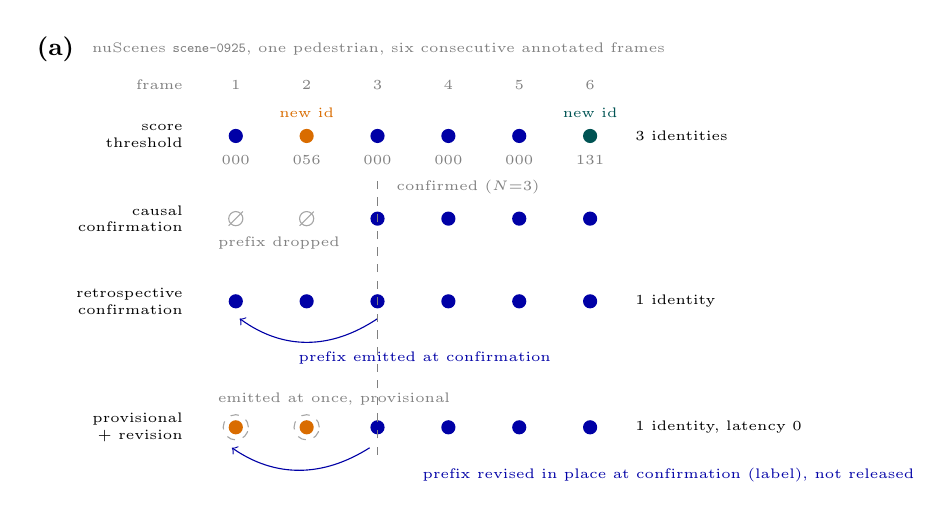
\begin{tikzpicture}
  \node[font=\small\bfseries, anchor=west] at (-1.75, 3.2) {(a)};
  \node[font=\tiny, gray, anchor=west] at (-1.05, 3.2) {nuScenes \texttt{scene-0925}, one pedestrian, six consecutive annotated frames};
  \foreach \x in {1,...,6} {\node[font=\tiny, gray] at (\x*0.9, 2.75) {\x};}
  \node[font=\tiny, gray, anchor=east] at (0.35, 2.75) {frame};
  % row 1: score threshold -- measured identities
  \node[anchor=east, align=right, font=\tiny] at (0.35, 2.1) {score\\threshold};
  \foreach \x in {1,3,4,5} {\fill[blue!65!black] (\x*0.9, 2.1) circle (0.09);}
  \fill[orange!85!black] (1.8, 2.1) circle (0.09);
  \fill[teal!65!black] (5.4, 2.1) circle (0.09);
  \foreach \x/\lab in {1/000, 2/056, 3/000, 4/000, 5/000, 6/131} {
    \node[font=\tiny, gray] at (\x*0.9, 1.79) {\lab};}
  \node[font=\tiny, orange!85!black] at (1.8, 2.40) {new id};
  \node[font=\tiny, teal!65!black] at (5.4, 2.40) {new id};
  \node[font=\tiny, anchor=west] at (5.85, 2.1) {3 identities};
  % row 2: causal confirmation
  \node[anchor=east, align=right, font=\tiny] at (0.35, 1.05) {causal\\confirmation};
  \foreach \x in {1,2} {
    \draw[gray!70] (\x*0.9, 1.05) circle (0.09);
    \draw[gray!70] (\x*0.9-0.09, 1.05-0.09) -- (\x*0.9+0.09, 1.05+0.09);}
  \foreach \x in {3,...,6} {\fill[blue!65!black] (\x*0.9, 1.05) circle (0.09);}
  \node[font=\tiny, gray, anchor=west] at (0.55, 0.74) {prefix dropped};
  % row 3: retrospective confirmation
  \node[anchor=east, align=right, font=\tiny] at (0.35, 0.0) {retrospective\\confirmation};
  \foreach \x in {1,...,6} {\fill[blue!65!black] (\x*0.9, 0.0) circle (0.09);}
  \node[font=\tiny, anchor=west] at (5.85, 0.0) {1 identity};
  \draw[->, blue!65!black] (2.7, -0.22) .. controls (2.1, -0.62) and (1.5, -0.62) .. (0.95, -0.22);
  \node[font=\tiny, blue!65!black] at (3.3, -0.72) {prefix emitted at confirmation};

  % row 4: provisional emission + revision (ours)
  \node[anchor=east, align=right, font=\tiny] at (0.35, -1.6) {provisional\\${+}$ revision};
  \foreach \x in {1,2} {\fill[orange!85!black] (\x*0.9, -1.6) circle (0.09);
                        \draw[dashed, gray!70] (\x*0.9, -1.6) circle (0.16);}
  \foreach \x in {3,...,6} {\fill[blue!65!black] (\x*0.9, -1.6) circle (0.09);}
  \node[font=\tiny, anchor=west] at (5.85, -1.6) {1 identity, latency 0};
  \draw[->, blue!65!black] (2.6, -1.86) .. controls (2.0, -2.24) and (1.4, -2.24) .. (0.85, -1.86);
  \node[font=\tiny, blue!65!black, anchor=west] at (3.15, -2.20)
       {prefix revised in place at confirmation (label), not released};
  \node[font=\tiny, gray, anchor=west] at (0.55, -1.24) {emitted at once, provisional};
  % confirmation marker
  \draw[dashed, gray] (2.7, -1.95) -- (2.7, 1.55);
  \node[font=\tiny, gray, anchor=west] at (2.82, 1.45) {confirmed ($N{=}3$)};
\end{tikzpicture}}
\\[4pt]
\resizebox{0.92\columnwidth}{!}{%
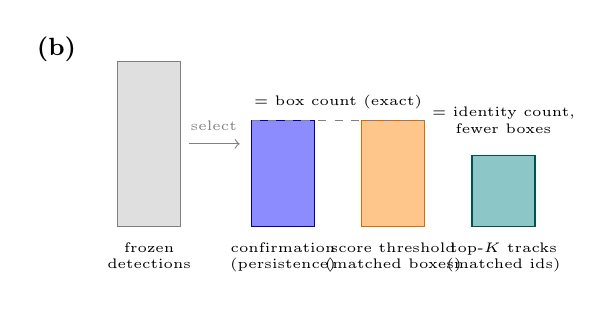
\begin{tikzpicture}
  \node[font=\small\bfseries, anchor=west] at (-1.15, 2.25) {(b)};
  \draw[fill=gray!25, draw=gray] (0, 0) rectangle (0.8, 2.1);
  \node[align=center, font=\tiny, anchor=north] at (0.4, -0.08) {frozen\\detections};
  \draw[->, gray] (0.9, 1.05) -- (1.55, 1.05);
  \node[font=\tiny, gray] at (1.22, 1.28) {select};
  \draw[fill=blue!45, draw=blue!65!black] (1.7, 0) rectangle (2.5, 1.35);
  \node[align=center, font=\tiny, anchor=north] at (2.1, -0.08) {confirmation\\(persistence)};
  \draw[fill=orange!45, draw=orange!85!black] (3.1, 0) rectangle (3.9, 1.35);
  \node[align=center, font=\tiny, anchor=north] at (3.5, -0.08) {score threshold\\(matched boxes)};
  \draw[fill=teal!45, draw=teal!65!black] (4.5, 0) rectangle (5.3, 0.9);
  \node[align=center, font=\tiny, anchor=north] at (4.9, -0.08) {top-$K$ tracks\\(matched ids)};
  \draw[dashed, gray] (1.7, 1.35) -- (3.9, 1.35);
  \node[font=\tiny] at (2.8, 1.58) {$=$ box count (exact)};
  \node[align=center, font=\tiny] at (4.9, 1.35) {$=$ identity count,\\fewer boxes};
\end{tikzpicture}}
\caption{\textbf{Emission policies over the same frozen detections.}
\textbf{(a)} Six consecutive annotated frames of nuScenes \texttt{scene-0925}
under a score threshold, causal confirmation, retrospective confirmation, and
our provisional emission with revision. Confirmation requires $N{=}3$; the
threshold carries no history and assigns three identities (last three digits
shown), while ours emits each observation immediately (dashed ring) and
revises its label after confirmation. \textbf{(b)} The detection- and
identity-budget controls match emitted boxes and emitted tracks respectively
(Sec.~\ref{sec:controls}).}
\label{fig:overview}
\end{figure}

% ---------------------------------------------------------------------------
% Fig. 1 goes here. Panel (a): four policy rows over the same six frames of
% nuScenes scene-0925 --- score threshold, causal confirmation, retrospective
% confirmation, provisional+revision. Panel (b): the matched-control diagram,
% unchanged. Caption:
%
% \caption{Emission policies over one frozen detection stream. (a) One
% pedestrian over six consecutive annotated frames of nuScenes
% \texttt{scene-0925}; all four rows select from the same frozen detections, so
% the emitted box is identical wherever a box is emitted at all and the rows
% differ only in \emph{when} a detection appears, under \emph{which} identity,
% and with \emph{which} label. A per-frame score threshold carries no history
% and assigns three identities to the object. Confirmation requires $N{=}3$
% observations: the \emph{causal} policy drops the pre-confirmation prefix, so
% the object first appears at its third observation; the \emph{retrospective}
% policy releases the withheld prefix at confirmation and recovers the whole
% trajectory under one identity, at the cost of emission latency. The
% \emph{provisional} policy emits every observation at its own frame (hollow
% markers, provisional status) and, at confirmation, revises the already
% emitted prefix in place (recoloured) instead of releasing it; a track that
% dies unconfirmed within the retraction horizon is retracted. (b) Every arm
% selects from the same frozen detection set; the detection-budget control is a
% score threshold calibrated to the module's exact box count, and the
% identity-budget control keeps the module's track count per sequence, which
% necessarily emits fewer boxes (Sec.~\ref{sec:controls}).}
% ---------------------------------------------------------------------------

\subsection{Temporal lifecycle}
\label{sec:pipeline}

Everything in this section is a post-processing operator over \emph{frozen}
detector output: no box coordinate or score is modified and no model is
retrained, and the operator's only freedoms are which detections enter the
output stream, under which persistent identity, with which label, and at which
frame. Per-frame detections --- a 3D box with a score and a class label --- are
linked across frames into tracks by a class-agnostic nearest-centroid
associator with a $2.0$\,m bird's-eye-view \textbf{association threshold} and a
\textbf{gap tolerance} of $5$ frames; no score threshold is applied before
association, and the associator is identical in every arm of every experiment.
Association runs either in the \emph{sensor frame} (raw detector coordinates)
or in the \emph{world frame} (ego-motion-compensated global coordinates), and
both are evaluated throughout, because ego-motion compensation changes how hard
association is. A track is \textbf{confirmed} once it has accumulated $N$
observations; we use $N{=}3$ throughout, the conventional setting in
tracking-by-detection systems, and do not tune it per dataset or per metric.
Counting is \emph{cumulative} over the scene rather than over consecutive
frames, so a track seen at frames $0,3,6$ confirms at frame $6$. An unconfirmed
track is \textbf{retracted} once $t - t_{\text{last seen}} > H$, where $H$ is
the \emph{retraction horizon} in frames; confirmed tracks are never retracted,
and $H{=}\infty$ applies no death rule and defers to a scene-end decision,
which serves as the reference endpoint.

\subsection{Emission policies}
\label{sec:emission}

Over an identical lifecycle, three policies differ only in what the consumer
sees and when (Fig.~\ref{fig:overview}a). \textbf{Causal confirmation} emits
nothing until confirmation and drops the pre-confirmation observations
permanently. \textbf{Retrospective confirmation} emits nothing until
confirmation, at which point the withheld prefix is released alongside the
current observation, completing the trajectory at the price of emission
latency. \textbf{Provisional emission with revision} (ours) emits every
observation at its own frame and revises it once the evidence completes.

\subsection{Provisional emission and revision}
\label{sec:latency}

Every observation is emitted at the frame it occurs under a \emph{provisional
status}: a flag on an emitted observation recording that the evidence
supporting it is not yet complete. It is a property of an emitted record, not
of a withheld one. Confirmation issues no prefix, because none was withheld;
it issues a \emph{revision} over the observations already delivered. In our
instantiation the revision rewrites the class label of the track's
already-emitted observations and the nuScenes attribute derived from it; box
geometry, detection score, and the persistent identity are not rewritten, so
the set of emitted boxes is unchanged by a revision. A track that reaches the
retraction horizon unconfirmed is retracted.

Retrospective confirmation incurs $N{-}1$ observations of latency, and a
larger empirical frame-index delay when observations contain gaps
(Sec.~\ref{sec:emissionabl}); our policy has zero emission latency --- asserted
mechanically, since every emitted record carries the frame index of its own
observation --- while $H$ bounds retraction rather than emission. What the
policy requires instead is a consumer that can act on an update to a record it
has already received.


% ---------------------------------------------------------------------------
% Edits to \section{Evaluation Protocol} (otherwise unchanged):
%
% [1] Sec. Metrics, Indoor: delete the seven-line vidstability/stability3d
%     digression ("Prediction stability has been measured separately ... in
%     that spirit for our setting.") and replace with:
%
%     Measuring prediction stability separately from accuracy has precedent in
%     video and 3D detection~\cite{vidstability,stability3d}, but that family
%     scores box trajectories against ground-truth tracks, which ScanNet200
%     does not provide, and none of it scores the \emph{class} assigned to a
%     persistent instance; we define the switch count in that spirit.
%
% [2] Sec. Statistics, final paragraph: replace the sentence beginning "the
%     evidence we offer for it is that its sign and rough magnitude are stable
%     across four independent comparisons (two controls $\times$ two
%     association frames)" with:
%
%     the evidence we offer for it is that its sign and rough magnitude are
%     stable across four independent detection-budget-matched cells ---
%     retrospective and causal emission, each in both association frames --- and
%     against both the score-threshold and the confidence-accumulation control.
%     We report no AMOTA under identity-budget matching, for the reason given
%     in Sec.~\ref{sec:discussion}.
% ---------------------------------------------------------------------------


\section{Evaluation Protocol}
\label{sec:protocol}

Every claim in this paper is made against a \emph{matched control} --- a
non-temporal selection rule granted the same output budget --- rather than
against the unfiltered baseline.

\subsection{Datasets and pipelines}
\label{sec:datasets}
\noindent\textbf{Outdoor.} The nuScenes~\cite{nuscenes} validation split, all
$150$ scenes at the $2$\,Hz annotated-frame rate. Detections come from a
pretrained CenterPoint~\cite{centerpoint} detector whose per-frame output is
computed once and \emph{frozen}; every arm of every experiment replays the
same stored detections ($718{,}786$ boxes over the split; mAP $0.5613$,
NDS $0.6480$).

\noindent\textbf{Indoor.} The ScanNet200~\cite{scannet200} validation split,
all $312$ scenes, in a streaming instance-segmentation pipeline: class-agnostic
3D instance-mask proposals from Mask3D~\cite{mask3d} are labeled per frame by a
2D open-vocabulary detector~\cite{yoloworld}, so each persistent instance
receives a stream of per-frame class labels. The proposal set is likewise
frozen across arms. This pipeline shares no detector, modality, or codebase
beyond the temporal module with the outdoor one.

\subsection{Matched controls}
\label{sec:controls}
Two budgets are matched --- emitted detections and emitted identities
(Fig.~\ref{fig:overview}b) --- and under each we compare the module against a
non-temporal score rule and against the other established temporal rule.

\noindent\textbf{Detection-budget-matched control.} A score threshold on the
frozen baseline detections is calibrated so the control emits \emph{exactly} as
many boxes as the temporal module --- $257{,}259$ in the sensor frame
(threshold $0.2214$), $517{,}566$ in the world frame ($0.1272$), both with zero
count error. The match is exact because the count is a step function of the
threshold whose breakpoints are the observed scores: the matched threshold is
the $K$-th largest observed score, ties resolved upward so the count never
exceeds $K$.

\noindent\textbf{Identity-budget-matched control.} Per sequence, the control
keeps the $K$ highest-scoring tracks (ranked by mean detection score), $K$
being the number of identities the temporal module emits there; counts match
exactly ($64{,}428$ tracks sensor, $108{,}225$ world). Five additional arms
select the same $K$ tracks \emph{at random} (five seeds), scored on association
accuracy, separating score-based selection from selection per se. The two
budgets cannot hold at once: at equal track count the control emits fewer boxes
than the module ($190{,}708$ vs.\ $360{,}309$ sensor; $608{,}168$ vs.\
$754{,}500$ world), because score-ranked tracks are shorter than
persistence-selected ones.

\noindent\textbf{Confidence-accumulation control.} To compare persistence
against confidence rather than against a static score, a third control
propagates a track score by constant decay and fuses it with each matched
detection score, following CBMOT's reported best update
rule~\cite{cbmot}; its parameters are transcribed from the authors' released
implementation, not tuned here, except that the gap tolerance is our
associator's rather than theirs, since the frozen association is shared by
every arm. A single threshold on the refined score is calibrated to the same
budget as the arm it is compared with, by the rule above, so this control is
matched under both budgets. Its trained score-regression variant is not
reproduced: it is fit on nuScenes and would give the control supervision no
other arm receives.

\noindent\textbf{Indoor control.} The identity-budget design transfers
directly: the control keeps the $K$ highest-scoring instances per scene, where
$K$ matches the temporal module's emitted-instance count ($10{,}413$ instances
in total; the control realizes $10{,}410$). Three
additional arms select $K$ instances \emph{at random} per scene (three seeds),
to separate the effect of score-based selection from that of selection per se.

\subsection{Metrics}
\label{sec:metrics}
\noindent\textbf{Outdoor.} Official nuScenes mAP and NDS on the emitted box
set; class-agnostic HOTA, AssA, DetA, detection recall (DetRe), and IDF1 via
TrackEval~\cite{hota,idf1}, with similarity
$\mathrm{sim}=\mathrm{clip}(1-d_{xy}/2.0,\,0,\,1)$ matching the associator's
$2.0$\,m threshold; and official class-aware AMOTA~\cite{nuscenes_tracking}
over the $7$ nuScenes tracking classes; the two families are reported side by
side.

\noindent\textbf{Indoor.} The primary endpoint is the per-scene
count of \emph{label switches}: frames in which a persistent instance's
emitted class label differs from its label in the previous frame \emph{in
which it was emitted}. Counting against the last emission rather than the
last frame is what makes the count comparable across arms, since the arms
emit on different frames. Prediction stability has precedent as a separate
axis in video and 3D detection~\cite{vidstability,stability3d}, but that
family scores box trajectories against ground-truth tracks, which ScanNet200
does not provide, and none of it scores the \emph{class} assigned to a
persistent instance. The secondary endpoint is instance-segmentation AP on the
final reconstruction.

\subsection{Statistics}
\label{sec:stats}
For all three main comparisons --- detection-budget-matched,
identity-budget-matched, and indoor --- the arms, the primary endpoint, and
the criterion for a negative result were fixed before the run in a
pre-registration released with the code. For the outdoor comparisons that criterion was that the association
gain hold in \emph{both} association frames with scene-bootstrap intervals
excluding zero, and that the dataset-level metrics (mAP, AMOTA) move
consistently across the two association frames, whichever direction they move
in; indoors,
that the per-scene label-switch count fall. The causal-emission ablation
(Sec.~\ref{sec:emissionabl}) predates that protocol and is what motivated it. All comparisons between the
temporal module and a control are paired per scene. We report the per-scene Wilcoxon signed-rank test with the
rank-biserial correlation as effect size, and a $95\%$ bootstrap confidence
interval on the difference of the aggregate metric obtained by resampling
scenes ($10{,}000$ resamples, fixed seed $20260718$). A difference is described as an
improvement only when its interval excludes zero; intervals that span zero are
reported as no detectable difference, whatever their sign.

Intervals are available for the class-agnostic metrics, which are defined
per scene and aggregate linearly over scenes. AMOTA is not, and neither are
the nuScenes devkit metrics mAP and NDS: AMOTA integrates MOTA over recall
thresholds estimated on the whole split, and mAP and NDS are likewise computed
over the whole split, so a per-scene resample does not yield the same
estimator. All three are reported as point estimates, and we claim no interval
support for AMOTA anywhere; the evidence we offer for it is that its sign and rough
magnitude are stable across four independent detection-budget-matched cells
--- retrospective and causal emission, each in both association frames --- and
against both the score-threshold and the confidence-accumulation control. The
two budgets cannot hold at once: matching emitted identities does not equalise
the identities reaching the class-aware evaluation, which scores a subset of
classes, so we report AMOTA only under detection matching.

\section{Experiments}
\label{sec:exp}

We report three outdoor comparisons on nuScenes val and one indoor comparison
on ScanNet200 val, each between the confirmation-based module and a control
granted the same output budget over shared frozen detections. Unless stated
otherwise, outdoor results use retrospective emission, whose latency cost is
$N{-}1$ observations; the corresponding frame-index delay is reported in
Sec.~\ref{sec:emissionabl}.

\subsection{Detection-budget-matched comparison}
\label{sec:detmatch}

\begin{table*}[t]
\centering\footnotesize
\setlength{\tabcolsep}{5pt}
\begin{tabular}{llrcccccccc}
\toprule
Frame & Arm & Boxes & mAP & NDS & HOTA & AssA & DetA & DetRe & IDF1 & AMOTA \\
\midrule
\multirow{4}{*}{Sensor}
 & Baseline (unfiltered)      &   718{,}786 & 0.5613 & 0.6480 & 0.1793 & 0.2007 & 0.1620 & 0.6690 & 0.1112 & 0.0858 \\
 & Control (threshold)       &   257{,}259 & \textbf{0.5504} & \textbf{0.6450} & \textbf{0.2735} & 0.2119 & \textbf{0.3570} & \textbf{0.6160} & 0.2082 & 0.0942 \\
 & Control (accumulation)     &   257{,}259 & 0.4783 & 0.6134 & 0.2604 & 0.2315 & 0.2954 & 0.5350 & 0.2146 & 0.1101 \\
 & Confirmation ($N{=}3$)     &   257{,}259 & 0.3009 & 0.5229 & 0.2462 & \textbf{0.2744} & 0.2232 & 0.4287 & 0.2054 & \textbf{0.1338} \\
\midrule
\multirow{4}{*}{World}
 & Baseline (unfiltered)      &   718{,}786 & 0.5613 & 0.6480 & 0.2837 & 0.5014 & 0.1613 & 0.6663 & 0.2715 & 0.2896 \\
 & Control (threshold)       &   517{,}566 & 0.5598 & 0.6479 & 0.3305 & 0.5146 & 0.2133 & 0.6550 & 0.3391 & 0.3137 \\
 & Control (accumulation)     &   517{,}565 & 0.5568 & 0.6467 & 0.3282 & 0.5110 & 0.2118 & 0.6511 & 0.3399 & 0.2931 \\
 & Confirmation ($N{=}3$)     &   517{,}566 & 0.4921 & 0.6200 & 0.3224 & \textbf{0.5293} & 0.1973 & 0.6141 & 0.3288 & \textbf{0.3864} \\
\bottomrule
\end{tabular}
\caption{\textbf{Detection-budget-matched comparison} on nuScenes val
($150$ scenes, frozen CenterPoint detections, retrospective emission). The
three matched arms --- a static score threshold ($0.2214$ sensor, $0.1272$
world), a confidence-accumulation control in the manner of~\cite{cbmot}, and
confirmation --- emit the same number of boxes. Bold marks the best
matched arm, omitted where the leading interval spans zero; the unfiltered
baseline is reference only and is not budget-matched.}
\label{tab:detmatch}
\end{table*}

Table~\ref{tab:detmatch} compares confirmation against controls calibrated to
the identical box count --- $257{,}259$ boxes in the sensor frame and
$517{,}566$ in the world frame, from the same frozen detector output.

\noindent\textbf{Association accuracy improves.} Against the threshold control
AssA rises from $0.2119$ to $0.2744$ in the sensor frame and from $0.5146$ to
$0.5293$ in the world frame, both intervals excluding zero
($[{+}0.0471,{+}0.0785]$ and $[{+}0.0098,{+}0.0203]$). The per-scene mean gain, a different estimator
from the difference of aggregates, is $+0.0460$; the gain holds in $113$ of
$150$ scenes
(Wilcoxon $p{=}2.6{\times}10^{-15}$, rank-biserial $0.74$).

\noindent\textbf{Class-aware tracking accuracy rises.} AMOTA goes from
$0.0942$ to $0.1338$ (sensor) and $0.3137$ to $0.3864$ (world), the largest
relative effect we measure. AMOTA admits no per-scene resampling
(Sec.~\ref{sec:stats}), so this is a point estimate that we rely on only
because it moves the same way in both frames and under the comparisons
below.

\noindent\textbf{Detection-oriented metrics fall.} At the same budget, mAP
drops $0.5504\!\to\!0.3009$ (sensor) and $0.5598\!\to\!0.4921$ (world), DetA
drops $0.3570\!\to\!0.2232$ ($[{-}0.1408,{-}0.1267]$) and
$0.2133\!\to\!0.1973$ ($[{-}0.0183,{-}0.0138]$), and detection recall drops
$0.6160\!\to\!0.4287$ ($[{-}0.2087,{-}0.1665]$) and $0.6550\!\to\!0.6141$
($[{-}0.0477,{-}0.0350]$). The DetA loss dominates the geometric mean, so
aggregate HOTA falls as well ($[{-}0.0323,{-}0.0231]$ sensor;
$[{-}0.0100,{-}0.0063]$ world).

\noindent\textbf{IDF1 shows no reliable sensor-frame difference.} The
sensor-frame interval spans zero ($[{-}0.0108,{+}0.0037]$) while the paired
per-scene test reaches significance ($p{=}7.3{\times}10^{-3}$), so the two
estimators disagree and we claim no difference; in the world frame IDF1 is
slightly \emph{lower} for the confirmation module
($[{-}0.0135,{-}0.0070]$).

\noindent\textbf{Against confidence accumulation, the two rules split the
metrics.} This control isolates \emph{which} temporal rule is used rather
than whether one is used at all. Confirmation attains higher AssA in both
frames
($0.2315\!\to\!0.2744$ sensor, $0.5110\!\to\!0.5293$ world; intervals
$[{+}0.0337,{+}0.0524]$ and $[{+}0.0146,{+}0.0225]$), and accumulation is ahead
on every other measured axis, also with intervals excluding zero: HOTA, DetA, IDF1 and DetRe
(Sec.~\ref{supp:cbmot}).
The split extends to detection quality: accumulation leads on mAP
($0.4783\!\to\!0.3009$ sensor, $0.5568\!\to\!0.4921$ world) and NDS
($0.6134\!\to\!0.5229$, $0.6467\!\to\!0.6200$).

\noindent\textbf{Scope of the accumulation control.} All statements about it
concern our reproduction under the configuration of Sec.~\ref{sec:controls},
not the original system or its published results
(Sec.~\ref{supp:cbmot}).

\subsection{Identity-budget-matched comparison}
\label{sec:idmatch}

\begin{table}[tb]
\centering\footnotesize
\setlength{\tabcolsep}{1.5pt}
\begin{tabular}{lrcccc}
\toprule
Arm & Boxes & HOTA & AssA & DetA & IDF1 \\
\midrule
\multicolumn{6}{l}{\emph{Sensor frame}} \\
Control (top-$K$)  & 190{,}708 & \textbf{0.2461} & 0.2346 & \textbf{0.2607} & \textbf{0.2081} \\
Control (rand.) & --- & --- &.2321--.2460 & --- & --- \\
Confirmation       & 360{,}309 & 0.1960 & \textbf{0.2535} & 0.1537 & 0.1531 \\
\midrule
\multicolumn{6}{l}{\emph{World frame}} \\
Control (top-$K$)  & 608{,}168 & \textbf{0.2538} & 0.4173 & \textbf{0.1553} & \textbf{0.2596} \\
Control (rand.) & --- & --- &.3878--.3934 & --- & --- \\
Confirmation       & 754{,}500 & 0.2263 & \textbf{0.4314} & 0.1196 & 0.2121 \\
\bottomrule
\end{tabular}
\caption{\textbf{Identity-budget-matched comparison.} The control keeps, per
scene, the $K$ highest-scoring tracks, $K$ being the number of identities the
confirmation module emits ($64{,}428$ sensor, $108{,}225$ world; exact in both
frames); the random-$K$ rows (``rand.'') give the range over five seeds of the
same selection made at random, scored on AssA only. The box budgets are
unequal here, in the control's disfavour on volume-sensitive metrics. AMOTA is
omitted: identity matching does not equalise class-aware evaluation volume
(Sec.~\ref{sec:stats}).}
\label{tab:idmatch}
\end{table}

Matching emitted identities rather than boxes
(Tab.~\ref{tab:idmatch}) tests whether the association gain merely reflects
having fewer identities to confuse. It does not. AssA remains higher for the
confirmation module in both frames ($0.2346\!\to\!0.2535$ sensor,
$0.4173\!\to\!0.4314$ world), with intervals excluding zero
($[{+}0.0129,{+}0.0258]$ and $[{+}0.0101,{+}0.0185]$) and per-scene wins in
$117/150$ and $111/150$ scenes ($p{=}2.2{\times}10^{-16}$ and
$4.1{\times}10^{-11}$). Selecting the same number of tracks \emph{at random}
rather than by score reproduces none of it: the seeded arms reach at most
$0.2460$ (sensor) and $0.3934$ (world), both below the confirmation module.

\noindent\textbf{The rule separation survives identity matching.} Repeating the
comparison against confidence accumulation with \emph{identities} rather than
boxes held fixed --- the accumulation control ranked by its own refined score
and cut at the confirmation module's per-scene identity count, matched exactly
--- leaves the association separation unchanged: $+0.0252$ sensor
($[{+}0.0200,{+}0.0316]$) and $+0.0172$ world ($[{+}0.0089,{+}0.0161]$),
against $+0.0253$ and $+0.0170$ at matched boxes, with the accompanying losses
on HOTA, DetA, IDF1 and DetRe keeping their sign and significance. The
separation is the same size whichever currency is held fixed, which excludes
the simplest reading of it --- that persistence gains association accuracy by
carrying fewer identities. The result is robust to the control's ranking and
matching granularity (Sec.~\ref{supp:ranking}).

\noindent\textbf{Budget asymmetry.} Identity matching necessarily leaves
unequal box counts, because score-ranked tracks are shorter than
persistence-selected ones. This biases volume-sensitive metrics against the
control --- so the AssA result here is conservative --- and we therefore read
DetA, HOTA and IDF1 from Tab.~\ref{tab:detmatch}, where boxes are matched
exactly.

\subsection{What the association gain is bought with}
\label{sec:emissionabl}

Sections~\ref{sec:detmatch} and~\ref{sec:idmatch} price confirmation in
detection retention. This section asks what \emph{else} it pays. All results so
far release a confirmed track's withheld prefix retrospectively; we first
measure the causal alternative, then a policy that avoids both costs.

\begin{table}[tb]
\centering\footnotesize
\setlength{\tabcolsep}{2.5pt}
\begin{tabular}{lrcccc}
\toprule
Arm & Boxes & mAP & HOTA & AssA & AMOTA \\
\midrule
\multicolumn{6}{l}{\emph{Sensor frame}} \\
Control (threshold)  & 221{,}297 & \textbf{0.3213} & \textbf{0.2417} & 0.2105 & 0.0574 \\
Confirmation, causal & 221{,}297 & 0.1360 & 0.2056 & \textbf{0.2861} & \textbf{0.0800} \\
\midrule
\multicolumn{6}{l}{\emph{World frame}} \\
Control (threshold)  & 503{,}619 & \textbf{0.3367} & \textbf{0.2729} & \textbf{0.4315} & 0.1825 \\
Confirmation, causal & 503{,}619 & 0.2569 & 0.2456 & 0.4199 & \textbf{0.2089} \\
\bottomrule
\end{tabular}
\caption{\textbf{Causal emission is not free either: detection-budget-matched}
($221{,}297$ boxes sensor at threshold $0.2519$, $503{,}619$ world at
$0.1539$; both arms exact). The causal arm drops the pre-confirmation prefix
instead of releasing it retrospectively. Intervals are reported for AssA only,
the metric the comparison turns on; the remaining columns are point
estimates.}
\label{tab:causal}
\end{table}

\noindent\textbf{Causal emission loses the prefix, and with it the world-frame
gain.} Table~\ref{tab:causal} repeats the detection-budget-matched comparison
with the prefix permanently dropped. The result splits by association frame.
The AMOTA gain survives in both ($0.0574\!\to\!0.0800$ sensor,
$0.1825\!\to\!0.2089$ world), and in the sensor frame the association gain is
not merely preserved but larger than under retrospective emission
($0.2105\!\to\!0.2861$; interval $[{+}0.0577,{+}0.0922]$ against
$[{+}0.0370,{+}0.0615]$ retrospectively, $110$ of $150$ scenes). In the world
frame, however, causal emission \emph{loses} association accuracy relative to
the control ($0.4315\!\to\!0.4199$), with a bootstrap interval entirely below
zero ($[{-}0.0183,{-}0.0047]$; paired $p{=}0.008$, rank-biserial $-0.25$,
confirmation ahead in only $53$ of $150$ scenes). The detection cost is larger
throughout than under retrospective emission (mAP $0.3213\!\to\!0.1360$
sensor).

Causal emission is worse where association was already easy: ego-motion
compensation leaves the world-frame control associating well on its own, and
there the discarded prefix costs more than confirmation cleans up.

\noindent\textbf{How much latency, in which unit.} The $N-1$ figure routinely
quoted for retrospective emission is correct only in observations
(Sec.~\ref{sec:latency}): over the $150$ scenes the confirmation \emph{frame}
horizon has median $3$ and $95$th percentile $7$ --- $1.5$\,s and $3.5$\,s at
the $2$\,Hz annotated-frame rate, against a constant $2$-observation horizon.
It is unbounded in principle (Sec.~\ref{supp:latency}).

\begin{table*}[t]
\centering\footnotesize
\setlength{\tabcolsep}{6pt}
\begin{tabular}{lrccccccc}
\toprule
Arm & Boxes & mAP & NDS & HOTA & AssA & DetA & IDF1 & AMOTA \\
\midrule
Baseline (ungated) & 718{,}786 & 0.5613 & 0.6480 & 0.2837 & 0.5014 & 0.1613 & 0.2715 & 0.2896 \\
Confirmation $N{=}3$ (prefix-deleting) & 368{,}724 & 0.4483 & 0.6013 & 0.3452 & 0.5265 & 0.2275 & 0.3662 & 0.4051 \\
\midrule
\multicolumn{9}{l}{\emph{Ours, provisional emission, retraction horizon $H{=}0$}} \\
\quad provisional & 295{,}403 & 0.3832 & 0.5651 & \textbf{0.3675} & \textbf{0.5619} & \textbf{0.2417} & \textbf{0.4198} & 0.3603 \\
\quad ${+}$ revision & 295{,}403 & 0.3950 & 0.5701 & --- & --- & --- & --- & 0.4200 \\
\midrule
\multicolumn{9}{l}{\emph{Ours, provisional emission, retraction horizon $H{=}4$}} \\
\quad provisional & 529{,}662 & 0.4927 & 0.6206 & 0.3219 & 0.5378 & 0.1936 & 0.3305 & 0.3823 \\
\quad ${+}$ revision & 529{,}662 & \textbf{0.5025} & \textbf{0.6247} & --- & --- & --- & --- & \textbf{0.4646} \\
\bottomrule
\end{tabular}
\caption{\textbf{Provisional emission and revision}, world frame, nuScenes val
($150$ scenes, $N{=}3$, same frozen detections and association as
Tab.~\ref{tab:detmatch}). These arms are \textbf{not budget-matched}: the box
count \emph{is} what the emission policy acts on. Revision changes no box,
score, or identity, so the class-agnostic metrics are \emph{identical} by
construction (``---''). Bold marks the best policy/confirmation value.}
\label{tab:policy}
\end{table*}

\noindent\textbf{Provisional emission retains the prefix at zero latency.}
Table~\ref{tab:policy} measures the proposed policy against the
prefix-deleting $N{=}3$ confirmation arm over the identical frozen stream. At a retraction
horizon of $H{=}4$ frames the policy emits $529{,}662$ boxes against that arm's
$368{,}724$: it retains $160{,}938$ observations ($+43.7\%$) that the arm
deletes, and it does so at an emission latency of exactly zero frames. Detection
quality on the emitted set rises accordingly (mAP $0.4483\!\to\!0.4927$, NDS
$0.6013\!\to\!0.6206$) and so does association consistency
(AssA $0.5265\!\to\!0.5378$).

\noindent\textbf{And it is not free.} Over the same comparison the policy
gives up class-agnostic detection and identity quality: DetA
$0.2275\!\to\!0.1936$, aggregate HOTA $0.3452\!\to\!0.3219$, IDF1
$0.3662\!\to\!0.3305$, and AMOTA before revision falls
$0.4051\!\to\!0.3823$. Emitting a provisional record means emitting records
that causal confirmation would have suppressed and that ground truth does not support, and
the class-agnostic metrics price exactly that.

\noindent\textbf{Revision recovers the class-aware endpoint.} Applying the
completed-evidence label to the already-emitted stream takes AMOTA
$0.3823\!\to\!0.4646$ at $H{=}4$ ($+0.0823$), leaving the net effect against
the prefix-deleting confirmation arm at $+0.0594$: revision restores, and then
exceeds, an AMOTA the emission step had lost rather than adding one on top of
it. It says nothing about association --- the class-agnostic matcher does not
read the class label, so those columns are a mechanical identity, not a null
result.

\noindent\textbf{The retraction horizon saturates.} $H$ prices how long a
provisional record may still be withdrawn. At $H{=}4$ the emitted output
becomes identical --- byte-identical, verified by checksum --- to the
unbounded $H{=}\infty$ policy that defers the decision to scene end, because no
track that ever confirms has a pre-confirmation gap wider than four frames.
Every endpoint at $H\!\ge\!4$ therefore coincides by output equality rather
than by a tuned metric match. The bound replaces the scene-end decision at no cost
in output (Sec.~\ref{supp:horizon}).

\noindent\textbf{The horizon is itself a trade-off.} Tightening it to $H{=}0$
--- retract at the first missed frame --- reverses the picture: the policy then
emits fewer boxes than the confirmation arm ($295{,}403$) and is the \emph{best} arm in the
table on every class-agnostic metric (AssA $0.5619$, HOTA $0.3675$, DetA
$0.2417$, IDF1 $0.4198$), while giving up mAP and AMOTA. We report both
endpoints rather than selecting the one that flatters a chosen column: $H$
buys retention and detection quality with class-agnostic identity quality,
and $H{=}4$ is the setting at which the unbounded-horizon result is recovered
in full at bounded latency.



\subsection{Confirmation-window sensitivity}
\label{sec:nsweep}

% Confirmation-window trade-off curve. Numbers are Tab. tab:nsweep (supplementary).
% Requires pgfplots (loaded in main.tex).
\begin{figure}[t]
\centering
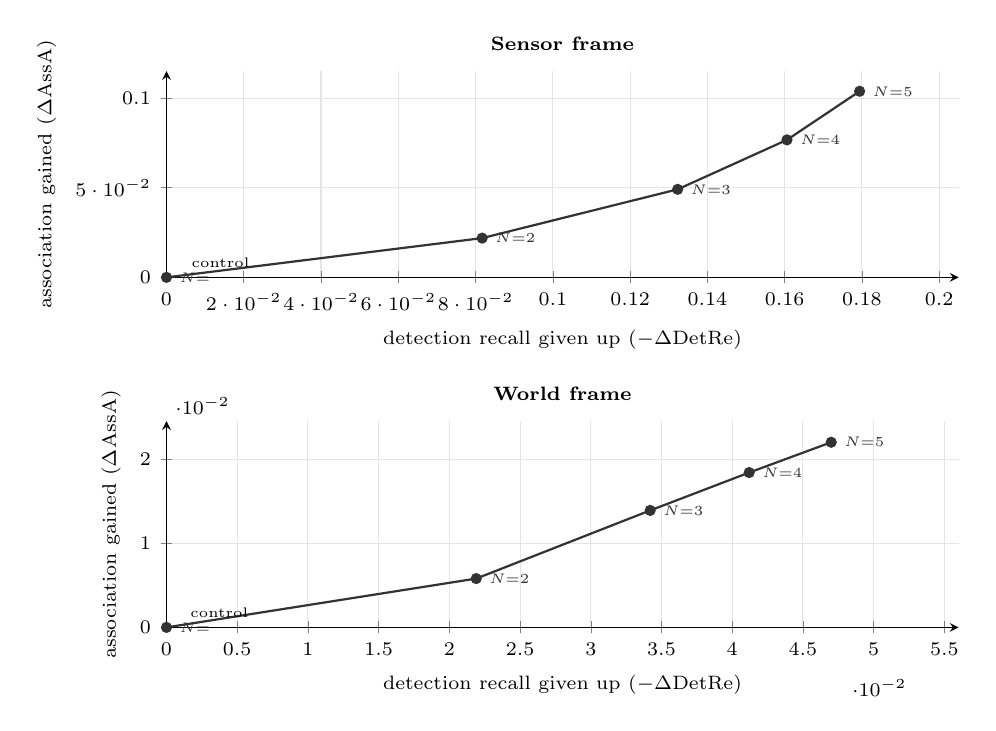
\begin{tikzpicture}
\pgfplotsset{
  every axis/.append style={
    width=0.96\linewidth, height=4.2cm,
    tick label style={font=\scriptsize}, label style={font=\scriptsize},
    title style={font=\scriptsize\bfseries, yshift=-2pt},
    axis lines=left, xmin=0, ymin=0,
    grid=major, grid style={gray!20},
  },
  every node near coord/.append style={font=\tiny, anchor=west, xshift=1pt},
}
\begin{axis}[
  name=sensor, title={Sensor frame},
  xmax=0.205, ymax=0.115,
  xlabel={detection recall given up ($-\Delta$DetRe)},
  ylabel={association gained ($\Delta$AssA)},
]
\addplot[thick, mark=*, mark size=1.6pt, color=black!80,
         nodes near coords={$N{=}\pgfplotspointmeta$}, point meta=explicit symbolic]
  coordinates {(0,0)[\!\!] (0.0817,0.0219)[2] (0.1323,0.0491)[3]
               (0.1606,0.0767)[4] (0.1794,0.1038)[5]};
\node[font=\tiny, anchor=south west] at (axis cs:0.004,0.0) {control};
\end{axis}
\begin{axis}[
  at={(sensor.below south west)}, anchor=north west, yshift=-8mm,
  title={World frame},
  xmax=0.056, ymax=0.0245,
  xlabel={detection recall given up ($-\Delta$DetRe)},
  ylabel={association gained ($\Delta$AssA)},
]
\addplot[thick, mark=*, mark size=1.6pt, color=black!80,
         nodes near coords={$N{=}\pgfplotspointmeta$}, point meta=explicit symbolic]
  coordinates {(0,0)[\!\!] (0.0219,0.0058)[2] (0.0342,0.0139)[3]
               (0.0412,0.0184)[4] (0.0470,0.0220)[5]};
\node[font=\tiny, anchor=south west] at (axis cs:0.001,0.0) {control};
\end{axis}
\end{tikzpicture}
\caption{\textbf{Confirmation is a trade-off curve, not a tuned setting.} Each
point is confirmation at that $N$ minus \emph{its own} detection-budget-matched
threshold control, so the control sits at the origin. Moving right along the
curve spends detection recall and $N{-}1$ frames of latency ($0.5$\,s each at
$2$\,Hz) and buys association accuracy; $N$ is chosen by the latency a
deployment can absorb rather than by a metric. The association gain is
positive at every $N$ in both frames and all eight bootstrap intervals exclude
zero. Full numbers, including intervals and $\Delta$AMOTA --- which, unlike
$\Delta$AssA, turns over inside the range --- are in the supplementary.}
\label{fig:nsweep}
\end{figure}


All results so far fix $N{=}3$. Figure~\ref{fig:nsweep} varies it over
$\{2,3,4,5\}$, giving each $N$ its own exactly matched control, and asks what
the choice is worth. $N{=}1$ is excluded: it reproduces the unfiltered baseline
detection-for-detection, so its matched control is the same box set and every
difference is zero by construction.

The association gain does not depend on the operating point. It is positive at
every $N$ in both association frames, and all eight intervals exclude zero. It
also grows monotonically with $N$, close to linearly in the sensor frame and
with visible deceleration in the world frame, while AMOTA flattens in the
sensor frame and turns over in the world frame, peaking at $N{=}4$
(Tab.~\ref{tab:nsweep}). The
detection cost, meanwhile, rises without turning over at any $N$ we measured,
and the latency rises linearly by construction.

No single $N$ in this range is best on every metric, and $N{=}3$ is not the
best on any of them. We report this rather than adjust the operating point:
re-selecting $N$ from the sweep would convert an inherited constant into a
value tuned on the test metrics, the practice the matched controls exist to
guard against. We keep $N{=}3$ because $N$ is a latency budget, not a tuned
hyperparameter: it is fixed by the $N{-}1$ observations of delay a deployment
can absorb. What the sweep establishes is that the consistency gain is a
property of confirmation over the whole range tested, not an artifact of one
setting, and that larger windows buy more of it at proportionally more
detection cost and latency. The widening gap is driven by the confirmed arm
rather than by a failing control, whose own AssA also rises as the matched
budget tightens (Tab.~\ref{tab:nsweep}).

\subsection{Indoor: semantic stability}
\label{sec:indoor}

\begin{table}[tb]
\centering\footnotesize
\setlength{\tabcolsep}{2pt}
\begin{tabular}{lrrcc}
\toprule
Arm & Inst. & Switches & AP & AP$_{50}$ \\
\midrule
Baseline (unfiltered)  & --- & --- & 0.1956 & --- \\
Control (top-$K$)      & 10{,}410 & 23{,}303 & 0.1926 & 0.2504 \\
Control (random $K$)   & --- & 23{,}275--23{,}288 & --- & --- \\
Confirmation ($N{=}3$) & 10{,}413 & \textbf{17{,}045} & 0.1954 & 0.2532 \\
\bottomrule
\end{tabular}
% TODO(pending indoor re-run): add a "Switches / opportunity" rate column.
% Denominator now logged by scripts/indoor_matched_control.py (n_obs_total -
% n_unique_total); it falls out of the indoor N-sweep run at no extra cost.
\caption{\textbf{Indoor comparison} on ScanNet200 val ($312$ scenes, frozen
Mask3D proposals with per-frame open-vocabulary labels). The primary endpoint
is the per-scene label-switch count (lower is better, bold); the control keeps
the $K$ highest-scoring instances per scene, $K$ matched to the confirmation
module's emitted-instance count, and the random-$K$ row spans three seeds
($23{,}275$, $23{,}277$, $23{,}288$). The AP columns are secondary and untested.
The unfiltered baseline is a validity anchor rather than an arm, and only its
AP was recorded, hence its empty cells.}
\label{tab:indoor}
\end{table}

The indoor experiment asks whether the same rule improves \emph{semantic}
stability in the pipeline of Sec.~\ref{sec:datasets}, which shares nothing with
the outdoor one. Against the identity-matched control, confirmation reduces label
switches from $23{,}303$ to $17{,}045$, a $26.9\%$ reduction at an essentially
equal instance budget ($10{,}413$ vs.\ $10{,}410$). The reduction is $18.0$ switches at the median
(Sec.~\ref{supp:indoor}) and holds in $309$ of $312$ scenes (Wilcoxon
$p{=}1.5{\times}10^{-52}$, rank-biserial $0.99$). The three random-$K$ arms are
indistinguishable from the score-ranked control and far from the confirmation
module, so the reduction is specific to temporal selection rather than to
emitting fewer instances by any rule.

The secondary endpoint shows no material change: AP $0.1954$ against $0.1956$
unfiltered and $0.1926$ for the control. Unlike outdoors, the indoor gain
therefore does not come at a measurable detection-quality cost --- the two
pipelines differ in whether the withheld detections carry segmentation mass,
and we report the difference in effect without claiming the outdoor trade-off
is avoidable in general.


\section{Discussion}
\label{sec:discussion}

\subsection{Confirmation is a trade-off, not a free gain}

Against an unfiltered baseline, temporal confirmation appears to improve
nearly every tracking metric. Against a non-temporal rule granted the same
output budget, most of that apparent improvement is the effect of emitting
less, and what survives is both sharper and smaller: association consistency
improves, and detection-oriented accuracy degrades over an \emph{identical}
box set. The gain is bought rather than added, and each additional observation
of delay buys more of it at proportionally more detection cost. Against
confidence accumulation the picture is a split rather than an ordering ---
persistence takes association consistency, accumulation keeps the detection-
and identity-oriented measures --- so the choice between them is a choice of
which axis a system is consumed along, not a ranking.

\subsection{Provisional emission changes the currency of the cost}

Confirmation must decide what to do with the observations that precede it, and
the classical rule offers only two answers: release them late, or drop them
and lose the world-frame association gain with them. Neither is compatible
with a consumer that must act immediately on output whose reliability improves
later. The policy's content is a separation --- \emph{when output becomes
available} is decoupled from \emph{when evidence becomes reliable} --- which
converts the currency of the cost from latency or retention into
revisability: the consumer must accept that a record it holds may be updated
or withdrawn, and the retraction horizon bounds how long that obligation
lasts. It is an operating-point change, not a new confirmation mechanism.

\subsection{Limitations}

\noindent\textbf{The revision endpoint is single.} AMOTA is the only
class-aware metric available to us; the class-agnostic family cannot respond
to a semantic-only change, and its invariance in Tab.~\ref{tab:policy} is
mechanical rather than a null result. Whether revision affects identity
consistency would need a class-aware association metric, which we do not have
and do not claim. Nor do we separate the label change from the nuScenes
attribute recomputation it entails, so the AMOTA gain is attributed to the
pair.

\noindent\textbf{Scope.} We do not measure what a downstream planner or mapper
pays to apply a revision or a retraction. The full tracking evaluation is
nuScenes only, over a single frozen CenterPoint detection set, so we make no
cross-detector claim; ScanNet200 has no instance-tracking ground truth, so the
indoor endpoint is label switching rather than an identity metric and tests
whether the confirmation rule transfers, not whether the streaming claim holds
there.

\section{Conclusion}
\label{sec:conclusion}

Temporal confirmation provides a genuine association-consistency gain under
matched detection and identity budgets, but the gain is coupled to detection
retention and to latency. Provisional emission separates immediate output from
evidence maturity: observations are emitted causally, then revised or retracted
as evidence accumulates. On nuScenes, $H{=}4$ retains $43.7\%$ more
observations than the prefix-deleting confirmation arm and revision raises
AMOTA by $0.0823$ over the provisional output. Against the prefix-deleting arm
the policy gives up class-agnostic detection and identity quality. On
ScanNet200 the same rule reduces class-label switching by $26.9\%$ at a matched
identity count.
Confirmation is therefore best understood as an operating point in a
detection--association--latency--revisability trade-off rather than a
uniformly better tracker.


\bibliographystyle{ieeenat_fullname}
\bibliography{main}

\end{document}
